\documentclass[10pt]{article}
\pdfminorversion=7
\usepackage[letterpaper,margin=.75in]{geometry}
\usepackage{amsmath,amssymb,booktabs,array,graphicx,float}
\usepackage{placeins}
\usepackage[round,authoryear]{natbib}
\usepackage[font=small,labelfont=bf]{caption}
\usepackage{xcolor,fancyhdr,microtype}
\usepackage[colorlinks=true,linkcolor=teal,citecolor=teal,urlcolor=teal]{hyperref}
\hypersetup{pdftitle={Monotone regression bands: simulation study},pdfauthor={}}
\definecolor{ink}{HTML}{25313D}
\definecolor{accent}{HTML}{007F78}
\pagestyle{fancy}\fancyhf{}\fancyhead[L]{\small Monotone regression bands}
\fancyhead[R]{\small Simulation study}\fancyfoot[C]{\thepage}
\setlength{\headheight}{14pt}\setlength{\parskip}{4pt}
\setlength{\parindent}{0pt}\setlength{\emergencystretch}{2em}
\makeatletter\setlength{\@fptop}{0pt}\makeatother
\graphicspath{{isotonic_results/}}
\title{\color{ink}Monotone regression bands\\[4pt]
  \large Isotonic COSI constructions and a simulation comparison}
\author{}\date{28 October 2026}
\begin{document}\maketitle
\vspace{-1.5em}
\begin{center}\small
12 settings $\times$ 4 sample sizes $\times$ 500 Monte Carlo replications\quad
Nominal level: $95\%$\quad COSI tuning: $\delta=0.30$
\end{center}
This study compares two COSI confidence-band constructions based on
isotonic estimators, an independent isotonic pilot, and block-count scales.
It compares simultaneous containment and finite interior band width across
smooth signals, flat regions, a jump, unequal local slopes, changing noise
variance, and heavy tails. The shaded-band illustrations use the first
replication at each sample size. Companion materials provide the R implementation, raw simulation records,
diagnostics, and figures.
\section{Data and simulation design}
We generate independent observations
$Y_i=f_0(X_i)+\xi_i$, $1\le i\le n$, and compare six procedures for a monotone regression band. The sample sizes are $n\in\{100,250,500,1000\}$, with 500 Monte Carlo replications for each of the twelve settings in Table~\ref{tab:isotonic-dgp}. The nominal level is $95\%$. This report describes the implemented constructions and their empirical behavior. All reported coverage values are Monte Carlo frequencies.

Write $z=x-1/2$, let $Z\sim N(0,1)$, and let $T_\nu$ have the Student $t$ distribution with $\nu$ degrees of freedom. For the skewed-error setting, define
\[
 P_a=\sqrt{a(a-2)}\left\{\frac{a-1}{a}V_a-1\right\},\qquad
 \mathbb P(V_a>v)=v^{-a}\quad(v\ge1),\qquad a=2.5.
\]
Thus $P_a$ has mean zero and variance one. Set
$c_{1.5}=\Phi^{-1}(3/4)/F_{t_{1.5}}^{-1}(3/4)$, so that $c_{1.5}T_{1.5}$ and $Z$ have the same interquartile range. Unless the table specifies otherwise, $X\sim\mathrm{Unif}(0,1)$ and the error-generating variable is independent of $X$. In setting~11, $S$ is Rademacher, $U\sim\mathrm{Unif}(0,1)$, and $S,U,Z$ are independent. All error distributions have mean zero; setting~12 has infinite variance.

\begin{table}[htbp]
\centering
\small
\setlength{\tabcolsep}{4pt}
\begin{tabular}{@{}r p{.31\linewidth} p{.22\linewidth} p{.32\linewidth}@{}}
\toprule
Setting & $f_0(x)$ & Covariate distribution & Error $\xi$ \\
\midrule
1 & $x$ & Uniform & $0.2Z$ \\
2 & $(e^{2x}-1)/(e^2-1)$ & Uniform & $0.2Z$ \\
3 & $1/2+4z^3$ & Uniform & $0.2Z$ \\
4 & $x$ & $\mathrm{Beta}(2,3)$ & $(0.1+0.4X)Z$ \\
5 & $x$ & Uniform & $0.2T_3/\sqrt3$ \\
6 & $x$ & Uniform & $0.2P_{2.5}$ \\
7 & $1/2$ & Uniform & $0.2Z$ \\
8 & $4(z_+)^2$ & Uniform & $0.2Z$ \\
9 & $\begin{cases}0.2+0.4z,&z\le0,\\0.2+1.6z,&z>0.\end{cases}$ & Uniform & $0.2Z$ \\
10 & $0.4x+0.6\mathbf1\{x\ge1/2\}$ & Uniform & $0.2Z$ \\
11 & $x$ & $1/2+S\sqrt U/2$ & $0.2Z$ \\
12 & $x$ & Uniform & $0.2c_{1.5}T_{1.5}$ \\
\bottomrule
\end{tabular}
\caption{The twelve monotone regression settings. Settings~7--12 probe flatness, unequal local slopes, a jump, a design density that vanishes linearly at the center, and errors without a second moment. Setting~8 has a flat region followed by a quadratic rise.}
\label{tab:isotonic-dgp}
\end{table}

The local-shape distinctions are motivated by \cite[Section~2.3, especially Example~2.3; Section~3.2; Appendix~A]{mallick2026generalized}. We record the empirical frequencies of underestimation, overestimation, and equality separately at every anchor for the split, pilot, and full-sample estimators. We also record how often an anchor lies outside a subsample's observed covariate range.

\subsection{One-replication illustrations}
Figures~\ref{fig:one-replication-1}--\ref{fig:one-replication-12} illustrate the
bands for the prespecified first replication in every setting, at
$n=100,250,500,1000$. The shaded region is cosi-m+ and the dashed red
boundaries show HulC. The black curve is the truth, the blue step curve is
the full-sample isotonic fit, and the gray points are the observations.
Datasets are not nested across sample sizes. All band boundaries on
$[0.1,0.9]$ are displayed, although extreme responses can fall outside
the vertical range. Companion figures give the corresponding cosi-m
rectangular enclosures. The constructions and width measurements are
described after the illustrations.


\begin{figure}[h]\centering
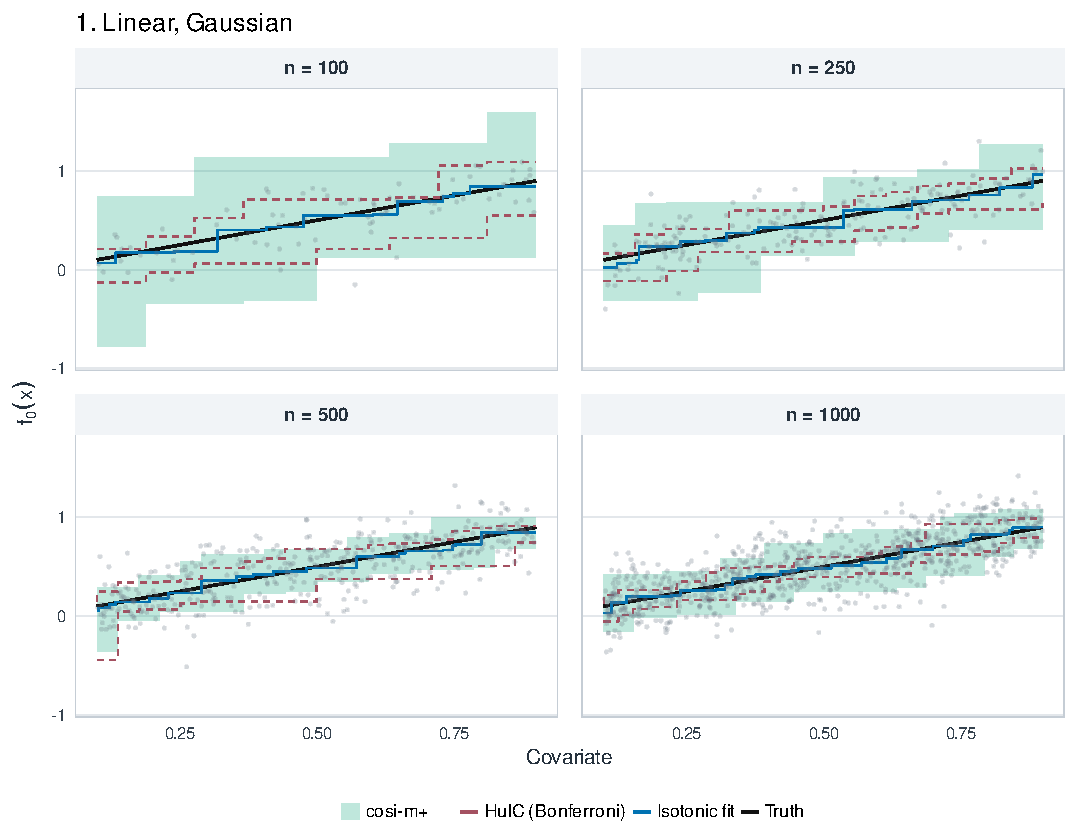
\includegraphics[page=1,width=\linewidth]{cosi_mplus_band_illustrations.pdf}
\caption{Setting 1: Linear mean, uniform covariates and Gaussian errors with standard deviation $0.2$.}
\label{fig:one-replication-1}
\end{figure}

\begin{figure}[h]\centering
\includegraphics[page=2,width=\linewidth]{cosi_mplus_band_illustrations.pdf}
\caption{Setting 2: Exponential mean, uniform covariates and Gaussian errors with standard deviation $0.2$.}
\label{fig:one-replication-2}
\end{figure}

\begin{figure}[h]\centering
\includegraphics[page=3,width=\linewidth]{cosi_mplus_band_illustrations.pdf}
\caption{Setting 3: Cubic mean with zero derivative at $1/2$, uniform covariates and Gaussian errors.}
\label{fig:one-replication-3}
\end{figure}

\begin{figure}[h]\centering
\includegraphics[page=4,width=\linewidth]{cosi_mplus_band_illustrations.pdf}
\caption{Setting 4: Linear mean with $\mathrm{Beta}(2,3)$ covariates and noise standard deviation $0.1+0.4x$.}
\label{fig:one-replication-4}
\end{figure}

\begin{figure}[h]\centering
\includegraphics[page=5,width=\linewidth]{cosi_mplus_band_illustrations.pdf}
\caption{Setting 5: Linear mean, uniform covariates and variance-normalized Student $t_3$ errors.}
\label{fig:one-replication-5}
\end{figure}

\begin{figure}[h]\centering
\includegraphics[page=6,width=\linewidth]{cosi_mplus_band_illustrations.pdf}
\caption{Setting 6: Linear mean, uniform covariates and centered, variance-normalized Pareto errors of shape $2.5$.}
\label{fig:one-replication-6}
\end{figure}

\begin{figure}[h]\centering
\includegraphics[page=7,width=\linewidth]{cosi_mplus_band_illustrations.pdf}
\caption{Setting 7: Constant mean $f_0=1/2$, uniform covariates and Gaussian errors.}
\label{fig:one-replication-7}
\end{figure}

\begin{figure}[h]\centering
\includegraphics[page=8,width=\linewidth]{cosi_mplus_band_illustrations.pdf}
\caption{Setting 8: Flat region followed by a quadratic rise, with uniform covariates and Gaussian errors.}
\label{fig:one-replication-8}
\end{figure}

\begin{figure}[h]\centering
\includegraphics[page=9,width=\linewidth]{cosi_mplus_band_illustrations.pdf}
\caption{Setting 9: Continuous kink with left and right slopes $0.4$ and $1.6$, with uniform covariates and Gaussian errors.}
\label{fig:one-replication-9}
\end{figure}

\begin{figure}[h]\centering
\includegraphics[page=10,width=\linewidth]{cosi_mplus_band_illustrations.pdf}
\caption{Setting 10: An increasing mean with a jump at $1/2$, where $f_0(1/2)=0.8$, with uniform covariates and Gaussian errors.}
\label{fig:one-replication-10}
\end{figure}

\begin{figure}[h]\centering
\includegraphics[page=11,width=\linewidth]{cosi_mplus_band_illustrations.pdf}
\caption{Setting 11: Linear mean with covariate density $4|x-1/2|$, which vanishes at the center, and Gaussian errors.}
\label{fig:one-replication-11}
\end{figure}

\begin{figure}[h]\centering
\includegraphics[page=12,width=\linewidth]{cosi_mplus_band_illustrations.pdf}
\caption{Setting 12: Linear mean, uniform covariates and Student $t_{1.5}$ errors scaled to match the Gaussian interquartile range.}
\label{fig:one-replication-12}
\end{figure}
\FloatBarrier

\section{Isotonic fits and the two COSI rectangles}
For each sample size, take $K=\lfloor\sqrt n\rfloor$ anchors equally spaced on $[0.1,0.9]$ and replace the anchor nearest $1/2$ by $1/2$. This gives $K=10,15,22,31$, respectively. The replacement ensures that the zero-derivative point, kink, and jump are evaluated directly. Every method uses this same deterministic grid.

An isotonic least squares fit minimizes $\sum_i\{Y_i-f(X_i)\}^2$ over nondecreasing $f$. The implementation sorts the pairs by $X$, aggregates tied covariates using their counts, and applies the pool-adjacent-violators calculation. Predictions are right-continuous steps: between adjacent observed covariates, use the fitted value at the covariate to the left. Beyond the observed covariate range, clamp to the first or last fitted value. This convention is used for every split and resample, including bootstrap samples with repeated pairs.

Randomly permute the observations and reserve $n_0=\lfloor n/2\rfloor$ observations in $S_0$ for the pilot. Split the remaining observations into $B=9$ balanced disjoint groups $S_1,\ldots,S_B$; this is the value returned by the calibration function \texttt{smallest\_B} at $\alpha=0.05$ and $\delta=0.30$. Define
\[
 \vartheta_k=\widehat f_{S_0}(t_k),\qquad
 W_{j,k}=\widehat f_{S_j}(t_k),\qquad
 s_k=\frac1{\sqrt{N_{0,k}}},
\]
where $N_{0,k}$ counts the original pilot observations in the constant PAVA block selected at $t_k$. At a clamped anchor, use the selected boundary block's count. At an observed covariate, this is the univariate selected-block count; at an off-design anchor we use the count associated with the stated step-extension convention. This is motivated by the selected-block quantity in \cite[Section~1.1, equations~(1.4) and~(1.6)]{deng2021confidence}. We use $s_k$ as a \emph{block-count normalization}, without multiplying by a residual standard deviation. The standard-error expression in their equation~(1.7) also includes a noise-scale estimate.

For clarity, the randomized cutoff $c^\star_{B,\beta}$ is implemented as follows. With $Z_B\sim\mathrm{Bin}(B,1/2)$, set
\[
 \begin{aligned}
 q&=\min\{r:\mathbb P(Z_B>r)\le\beta\},\\
 p&=\frac{\mathbb P(Z_B>q-1)-\beta}{\mathbb P(Z_B=q)},\\
 c^\star_{B,\beta}&=q-\mathbf1\{U>p\},
 \end{aligned}
\]
where $U\sim\mathrm{Unif}(0,1)$. Draw
$c_m=c^\star_{B,\alpha/2}$ and $c_+=c^\star_{B,\alpha}$ independently, using one realization of each cutoff for all anchors. Both cutoffs take values in $\{6,7\}$ in this study.

\paragraph{The rectangular cosi-m+ construction.}
Let $D_{j,k}=|W_{j,k}-\vartheta_k|/s_k$, and let $D_{(r),k}$ denote the $r$th order statistic over the $B$ splits at coordinate $k$. Set
\[
 R_+=\max_{1\le k\le K}D_{(c_++1),k},\qquad
 I^+_k=[\vartheta_k-R_+s_k,\ \vartheta_k+R_+s_k].
\]
The order statistic is taken \emph{before} the maximum over coordinates. In particular, this is not the order statistic of the splitwise maximum distances.

\paragraph{The rectangular enclosure of cosi-m.}
Set
$L_k=W_{(B-c_m),k}$ and $U_k=W_{(c_m+1),k}$. The selected-coordinate set uses
$k_\theta=\min\arg\max_k|\vartheta_k-\theta_k|/s_k$ and the condition $\theta_{k_\theta}\in[L_{k_\theta},U_{k_\theta}]$. We first take its closed coordinatewise rectangular enclosure. Write
\[
 r_k=\frac{\max\{|L_k-\vartheta_k|,|U_k-\vartheta_k|\}}{s_k},\qquad
 R_{-k}=\max_{\substack{\ell\ne k\\r_\ell>0\ \mathrm{or}\ \ell=1}}r_\ell,
\]
with $\max\varnothing=-\infty$. The enclosure has endpoints
\[
 \ell^m_k=\min\{L_k,\vartheta_k-s_kR_{-k}\},\qquad
 u^m_k=\max\{U_k,\vartheta_k+s_kR_{-k}\}.
\]
The eligibility condition handles the degenerate zero-radius tie. In the figures, \texttt{cosi-m (rectangle)} denotes this enclosure. Its reported width is the width of the associated monotone band; the nonrectangular selected-coordinate set is not used to calculate these widths. Because $c_m$ and $c_+$ use different levels and separate draws, the two reported rectangles need not be nested.

\section{From anchor rectangles to bands and width measurements}
For any method's anchor endpoints $(\ell_k,u_k)$, apply monotone tightening
\[
 A_k=\max_{i\le k}\ell_i,\qquad D_k=\min_{i\ge k}u_i.
\]
At $t_k$, the band is $[A_k,D_k]$; for $t_k<x<t_{k+1}$, it is $[A_k,D_{k+1}]$. To the left of $t_1$ the lower endpoint is $-\infty$, and to the right of $t_K$ the upper endpoint is $+\infty$. This uses the envelope construction of \cite{kuchibhotla2024hulc}; the explicit two-anchor formula is equation~(35), Section~5.3, pp.~27--28 of arXiv:2105.14577v2.

The finite width reported in the comparisons is the average height over the anchor span:
\[
 \overline w=\frac1{0.8}\sum_{k=1}^{K-1}(t_{k+1}-t_k)(D_{k+1}-A_k).
\]
It is not the average of the $K$ pointwise widths. The unbounded tails are outside the displayed and integrated domain $[0.1,0.9]$. If any $A_k>D_k$, the band is flagged as empty, its recorded width is zero, and its coverage indicator is false. No replication is discarded or redrawn. The empirical simultaneous-coverage indicator checks all $K$ tightened anchor intervals. Width ratios divide $\overline w$ by the HulC band's width from the same replication, before computing boxplots or medians.

\section{Full-sample comparison procedures}
The four benchmarks use all $n$ observations. Let $\widehat f_n(t_k)$ be the full-sample isotonic estimate. The bootstrap and subsampling calculations use the same pilot scales $s_k$ as COSI, held fixed during resampling. All supremum-root critical values use R's \texttt{quantile(type=6)}.

\paragraph{Pairs bootstrap.}
Draw 500 samples of $n$ pairs with replacement and refit isotonic regression. For each bootstrap fit $\widehat f_n^{*r}$, compute
\[
 T_r^*=\max_k\frac{|\widehat f_n^{*r}(t_k)-\widehat f_n(t_k)|}{s_k}.
\]
If $q^*$ is the empirical $0.95$ quantile, use the anchor intervals $[\widehat f_n(t_k)\pm q^*s_k]$, followed by the same monotone envelope. This is a supremum-distance pairs-bootstrap band, not coordinatewise percentile intervals.

\paragraph{Subsampling with rate $1/3$.}
Draw 500 subsets of $b=\operatorname{round}(n^{2/3})$ pairs without replacement. Each subset produces an isotonic fit $\widehat f_b^{\,r}$. If $q_b$ is the empirical $0.95$ quantile of
$\max_k|\widehat f_b^{\,r}(t_k)-\widehat f_n(t_k)|/s_k$, use the intervals
$[\widehat f_n(t_k)\pm (b/n)^{1/3}q_bs_k]$ and then tighten them. The resampling structure follows \cite[Chapter~2, pp.~39--64]{politis1999subsampling}.

\paragraph{Subsampling with estimated coordinatewise rates.}
Use 200 additional random subsets at each distinct feasible size
$b_j=\operatorname{round}(n^{\beta_j})$, with
$\beta_j\in\{0.9,0.75,0.6,0.45\}$ and $8\le b_j<n$. At each anchor, calculate four quantile ranges using probability pairs $(0.1,0.6)$, $(0.2,0.7)$, $(0.3,0.8)$, and $(0.4,0.9)$. The quantiles are obtained by inverting the empirical CDF on a 100-point grid spanning the observed values. Regress the mean of the four log ranges on $\log b_j$; the negative slope is $\widehat\gamma_k$. This follows the quantile-range approach of \cite{bertail1999subsampling}; see also \cite[Chapter~8, pp.~173--187]{politis1999subsampling}. The numerical grids and resample counts are the choices made for this simulation.

Reuse the same 500 construction subsets as the fixed-rate method and form
\[
 \widehat T_r=\max_k (b/n)^{\widehat\gamma_k}
   \frac{|\widehat f_b^{\,r}(t_k)-\widehat f_n(t_k)|}{s_k}.
\]
Thus the rate adjustment precedes the maximum. With $\widehat q$ its empirical $0.95$ quantile, use $[\widehat f_n(t_k)\pm\widehat q s_k]$ and tighten. Finite estimated rates, including negative values, are retained without clipping. A degenerate quantile range, a nonfinite regression result, or fewer than two usable sizes triggers a flagged fallback $\widehat\gamma_k=0$ at that coordinate.

\paragraph{HulC with a Bonferroni allocation.}
Use one balanced random partition of the full sample into
$B_H=\lceil\log_2(2K/\alpha)\rceil$ groups, giving $B_H=9,10,10,11$ at the four sample sizes. At each anchor, take the minimum and maximum of the $B_H$ isotonic estimates and apply the monotone envelope. The number of groups is deterministic; it is not randomized between adjacent integers.

\paragraph{Reproducibility and saved records.}
For setting $s$, sample size $n$, and replication $r$, the data seed is
$100+10^6s+10^3n+r$. The COSI split/cutoff stream uses this seed plus $5\times10^7$, and the benchmark stream uses it plus $10^8$. R's random-number algorithms are fixed to \texttt{Mersenne-Twister}, \texttt{Inversion}, and \texttt{Rejection}. Every method uses the same data within a replication. The illustrations use the prespecified first replication, $r=1$, at each sample size. The companion materials include band records, rate diagnostics, seeds, and source hashes. At $95\%$ coverage, 500 independent replications give a Monte Carlo standard error of approximately one percentage point. Coverage figures use panel-specific lower limits and a common upper limit of $101\%$, retaining every empirical coverage value. The vertical scales are labeled separately in each panel.

\section{Observed coverage and width}
The study comprises 24,000 simulated datasets and 144,000 method-level
band records. Each setting and sample-size combination includes 500 replications for
every method. No empty bands occurred, and no datasets were redrawn or removed.

Across the 44 cells with a continuous mean function, empirical coverage of
cosi-m+ ranges from 97.2\% to 100.0\%; at $n=1000$, it ranges from 98.4\%
to 100.0\%. The corresponding range for the cosi-m rectangular enclosure
over all four sample sizes is 98.2\% to 100.0\%. These values describe
simultaneous containment of all anchors and their monotone envelope.
The two COSI bands are frequently conservative in the tested continuous settings.
Their widths must therefore be read together with their coverage.

For the linear Gaussian setting, the median average width of cosi-m+ decreases
from 1.032 at $n=100$ to 0.440 at $n=1000$.
Its median paired width ratio relative to HulC changes from 1.962
to 1.917. The COSI methods reserve half of the sample for the pilot;
the HulC benchmark fits its blocks using the full sample. The comparison thus
includes the cost of that pilot allocation. Across the continuous settings,
the median paired cosi-m+/HulC ratios range from 1.551 to 2.336.
Table~\ref{tab:widths} reports the largest-sample widths and paired ratios.

The benchmark methods have distinct empirical behavior. In the linear Gaussian
setting at $n=1000$, coverage is 95.2\% for pairs bootstrap,
96.8\% for fixed-rate subsampling, 80.6\% for estimated-rate
subsampling, and 95.8\% for HulC. Under skewed Pareto errors, the
corresponding values are 97.8\%, 92.2\%, 99.2\%, and
83.8\%, compared with 99.8\% for cosi-m+.
These comparisons apply to the resampling and splitting implementations specified above.

Flatness and local asymmetry are visible in the sign diagnostics.
For the constant function at $n=1000$, the fraction of inference-block estimates
above the truth ranges from 0.195 to 0.780 across the anchors;
at $1/2$ it is 0.486. For the unequal-slope setting, the center fraction
is 0.608. The full sign-frequency curves are provided in the companion diagnostic figures.
These finite-sample sign frequencies are measured directly, without imposing
median balance on the split estimates.

The jump setting behaves differently. cosi-m+ coverage changes from 88.2\%
at $n=100$ to 70.2\% at $n=1000$; HulC coverage is 0.0\% at the
largest sample size. The target at the jump is $f_0(1/2)=0.8$, while the
off-design prediction convention selects the fitted value at the last observed
covariate at or below $1/2$. This is a deliberate discontinuity and point-value
stress experiment. Its numerical results are sensitive to that convention and
should be interpreted as such.

The estimated-rate comparison retains a separate exponent at every anchor.
An explicit zero-rate fallback was used at one or more anchors in 2.1\%
of replications. The companion diagnostics include coordinatewise median rates,
their 10th and 90th percentiles, and the fallback frequency. No finite exponent
was truncated to a prescribed range.

\subsection{Interpreting the pairs-bootstrap results}
Ordinary pairs resampling of the isotonic least squares estimator is
inconsistent in the usual pointwise cube-root setting; see
\cite[Section~1]{groeneboom2024confidence}. The linear Gaussian setting
already belongs to this regime, so unusual error distributions are not
needed for this issue to arise. The empirical resampling scheme does
not reproduce the deterministic local drift governing the sampling distribution.
Good coverage in some finite-sample experiments does not resolve this
distributional problem.

The present comparison assesses a symmetric maximum-absolute-distance
band over $K=\lfloor\sqrt n\rfloor$ anchors at a single nominal level.
It does not compare conditional pointwise bootstrap distributions with
their sampling distributions. Failure to estimate a distribution
consistently does not require substantial undercoverage at every
confidence level and sample size. Taking absolute values and a maximum
changes the statistic being assessed; those operations do not establish
consistency of the bootstrap band. Across the continuous-function
settings, its empirical coverage ranges from $90.8\%$ (setting~4,
$n=100$) to $99.2\%$ (setting~7, $n=1000$). In setting~11 it ranges
from $92.4\%$ to $93.2\%$ across the four sample sizes. Thus its
performance includes undercoverage as well as conservatism.

The jump setting gives bootstrap coverage between $24.8\%$ and
$32.6\%$, but estimation at the discontinuity and the prediction
convention are additional complications there. That example does not
isolate bootstrap inconsistency. For monotone truth, tightening the
anchor intervals preserves the simultaneous-containment event, so the
monotone envelope itself cannot explain the favorable bootstrap coverage.
A more direct distributional diagnostic would fix an interior point in
the linear Gaussian setting and compare bootstrap and sampling quantiles
over increasing sample sizes and several confidence levels. The current
results describe the implemented band and do not establish that ordinary
pairs bootstrap generally works for isotonic regression.

\subsection{Interpreting the width comparison with HulC}
HulC has the smaller median width in all 48 setting/sample-size cells,
but there is no ordering in every replication. The cosi-m rectangular
band is narrower than HulC in 278 of the 24,000 paired datasets
($1.16\%$), and cosi-m+ is narrower in 387 ($1.61\%$).

The comparison includes a substantial difference in data allocation.
COSI reserves half the observations for the pilot, leaving approximately
$n/18$ observations per inference block, whereas HulC uses approximately
$n/B_H$ per block, with $B_H\in\{9,10,11\}$. As a scale heuristic in
a regular positive-slope cube-root regime, this suggests a factor
$(18/B_H)^{1/3}$, between $1.18$ and $1.26$, for the pointwise estimation
scales. This calculation is not a decomposition of the observed band
widths and does not explain the full difference, which is often close to
a factor of two.

The Bonferroni allocation is implemented through the number of HulC
blocks, $B_H=\lceil\log_2(2K/\alpha)\rceil$, which changes only from
$9$ to $11$ over the grids considered here. It does not multiply the
band width by $K$. The Bonferroni label therefore does not determine
the width ordering relative to these COSI constructions.

The constructions also differ geometrically. In cosi-m+, the maximum of
the coordinatewise distance order statistics determines a common radius that is
then applied at every anchor. HulC uses each anchor's own minimum and
maximum. For cosi-m, the plotted band is based on the rectangular
enclosure of the selected-coordinate set: the enclosure discards the
set's restrictions coupling coordinates, and a large standardized radius
at one anchor can enlarge intervals at other anchors. These features can
contribute to wider bands; they do not imply deterministic containment
of one method's band in another. All methods use the same monotone
extension and the same integrated-width definition.

Finally, the empirical coverages are not matched. At $n=1000$ in the
linear Gaussian setting, HulC has median width $0.231$ and coverage
$95.8\%$, compared with median widths $0.464$ and $0.440$ for cosi-m
and cosi-m+, both with $100\%$ coverage. Under skewed Pareto errors,
HulC and cosi-m+ have coverage $83.8\%$ and $99.8\%$, respectively;
for the constant function the corresponding values are $86.0\%$ and
$99.6\%$. The narrower HulC bands therefore reflect a combination of
data allocation, band geometry, and different coverage behavior. The
present simulation does not separate their individual contributions.

\section{Numerical summaries at \texorpdfstring{$n=1000$}{n=1000}}
\begin{table}[H]\centering\small
\begin{tabular}{@{}r rrrrrr@{}}\toprule
Setting & cosi-m & cosi-m+ & HulC & Pairs & Sub.\ $(1/3)$ & Sub.\ est.\\\midrule
1 & 100.0 & 100.0 & 95.8 & 95.2 & 96.8 & 80.6 \\
2 & 100.0 & 100.0 & 96.4 & 95.4 & 95.6 & 79.2 \\
3 & 100.0 & 100.0 & 92.6 & 96.4 & 98.6 & 85.2 \\
4 & 100.0 & 99.8 & 94.8 & 94.6 & 97.4 & 95.6 \\
5 & 99.4 & 99.6 & 97.6 & 95.2 & 95.6 & 92.6 \\
6 & 100.0 & 99.8 & 83.8 & 97.8 & 92.2 & 99.2 \\
7 & 100.0 & 99.6 & 86.0 & 99.2 & 100.0 & 96.6 \\
8 & 100.0 & 100.0 & 90.8 & 93.8 & 98.4 & 87.8 \\
9 & 100.0 & 100.0 & 96.8 & 93.6 & 96.6 & 82.2 \\
10 & 72.4 & 70.2 & 0.0 & 24.8 & 52.8 & 19.4 \\
11 & 100.0 & 99.8 & 91.4 & 92.4 & 93.6 & 82.6 \\
12 & 98.6 & 98.4 & 96.6 & 96.2 & 93.4 & 99.4 \\
\bottomrule\end{tabular}
\caption{Empirical simultaneous coverage at $n=1000$, in percent, from 500
replications per setting. cosi-m denotes its rectangular enclosure. The nominal
level is $95\%$; the entries are empirical frequencies.}
\label{tab:coverage}\end{table}

\begin{table}[H]\centering\small
\begin{tabular}{@{}r rrrrr@{}}\toprule
& \multicolumn{3}{c}{Median average band width}
& \multicolumn{2}{c}{Median paired ratio to HulC}\\
\cmidrule(lr){2-4}\cmidrule(l){5-6}
Setting & cosi-m+ & HulC & Pairs & cosi-m & cosi-m+\\\midrule
1 & 0.440 & 0.231 & 0.242 & 2.001 & 1.917 \\
2 & 0.419 & 0.221 & 0.232 & 2.013 & 1.914 \\
3 & 0.352 & 0.183 & 0.188 & 2.063 & 1.942 \\
4 & 0.675 & 0.343 & 0.398 & 2.078 & 1.961 \\
5 & 0.432 & 0.224 & 0.245 & 1.988 & 1.921 \\
6 & 0.402 & 0.192 & 0.239 & 2.144 & 2.081 \\
7 & 0.161 & 0.093 & 0.060 & 1.928 & 1.753 \\
8 & 0.359 & 0.186 & 0.183 & 2.054 & 1.951 \\
9 & 0.435 & 0.225 & 0.233 & 2.024 & 1.930 \\
10 & 0.537 & 0.218 & 0.215 & 2.735 & 2.474 \\
11 & 0.537 & 0.267 & 0.286 & 2.145 & 2.030 \\
12 & 0.967 & 0.573 & 0.580 & 1.712 & 1.656 \\
\bottomrule\end{tabular}
\caption{Widths at $n=1000$. Average width is the integral of band height over
$[0.1,0.9]$, divided by $0.8$. The last two columns are medians of within-replication
ratios; they are not ratios of median widths. All methods' absolute widths and
paired ratios are provided in the companion numerical summaries and figures.}
\label{tab:widths}\end{table}
\FloatBarrier
\section{Empirical coverage comparisons}
Figures~\ref{fig:coverage-1}--\ref{fig:coverage-3} compare simultaneous
coverage as the sample size increases. Each panel retains all empirical
values, with a separate vertical range and a common nominal reference
of $95\%$. Coverage should be read together with the width comparisons
that follow.
\begin{figure}[h]\centering
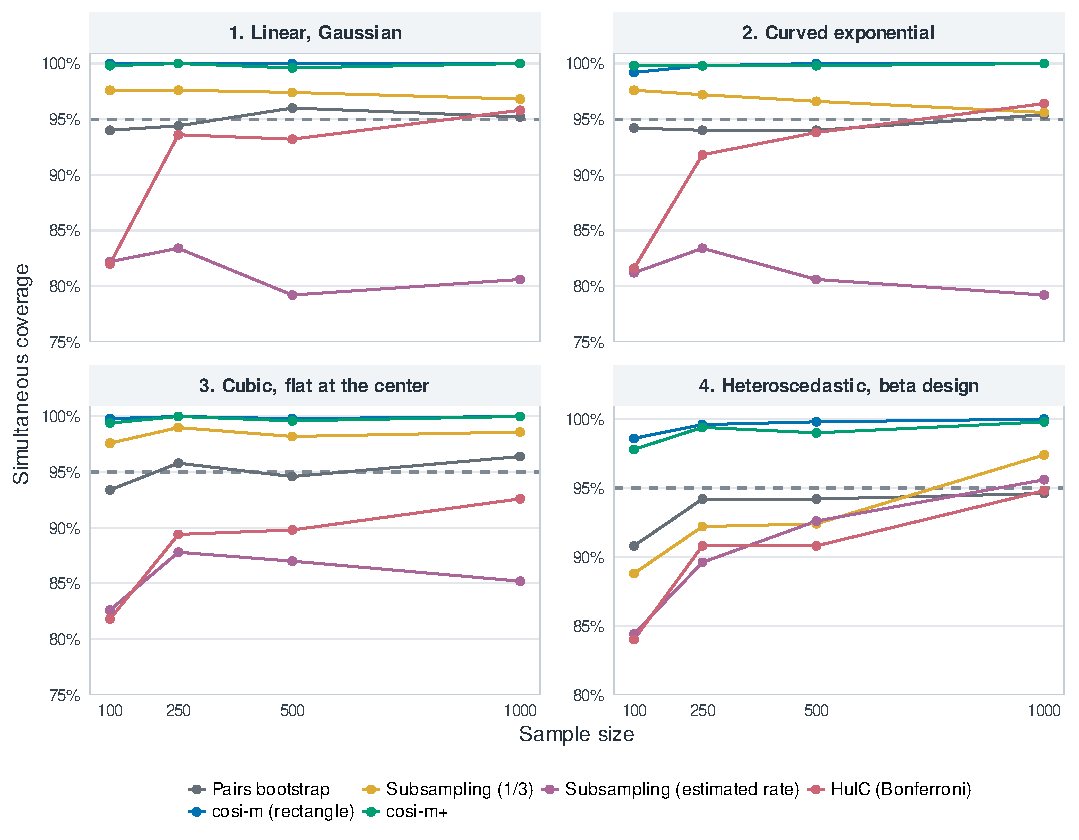
\includegraphics[width=\linewidth]{empirical_coverage_group_1.pdf}
\caption{Empirical simultaneous coverage for settings 1--4. The same data are
used for all methods within each of 500 replications at every sample size.
The dashed line marks the nominal $95\%$ level. Panel-specific vertical
limits retain all coverage values. Each rectangle is extended using the same
monotone envelope; every anchor is checked when recording coverage.}
\label{fig:coverage-1}
\end{figure}

\begin{figure}[h]\centering
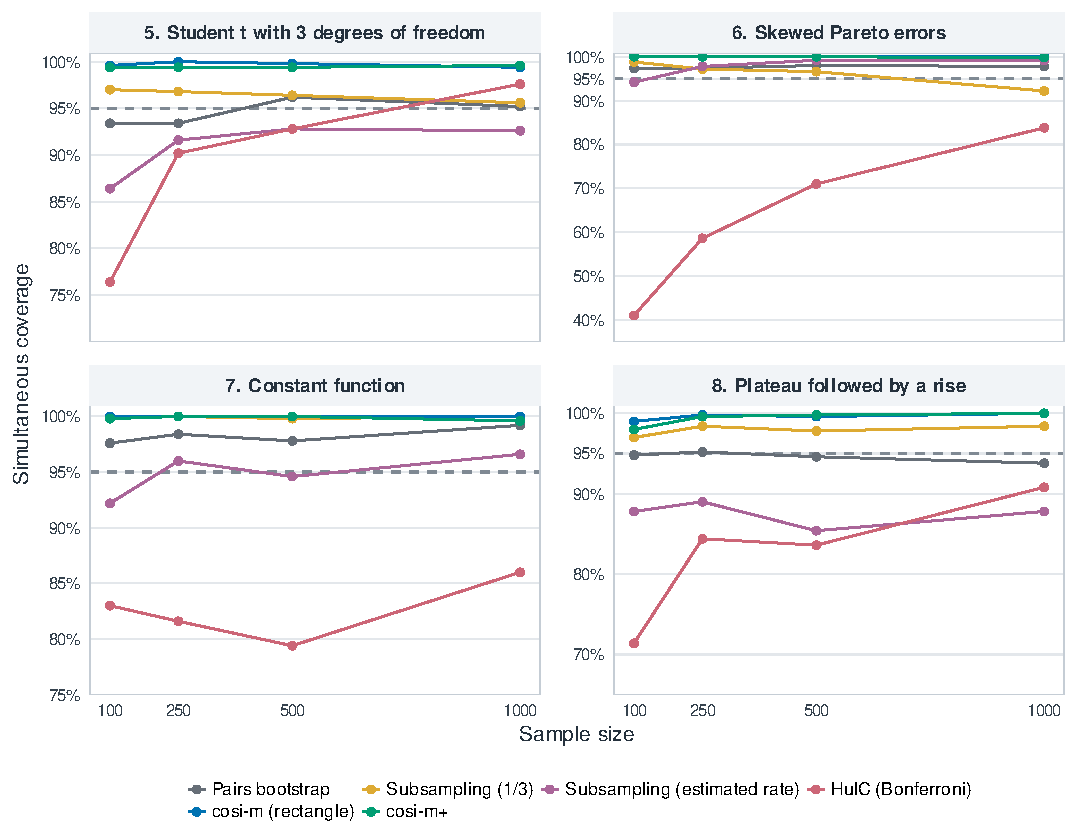
\includegraphics[width=\linewidth]{empirical_coverage_group_2.pdf}
\caption{Empirical simultaneous coverage for settings 5--8. The same data are
used for all methods within each of 500 replications at every sample size.
The dashed line marks the nominal $95\%$ level. Panel-specific vertical
limits retain all coverage values. Each rectangle is extended using the same
monotone envelope; every anchor is checked when recording coverage.}
\label{fig:coverage-2}
\end{figure}

\begin{figure}[h]\centering
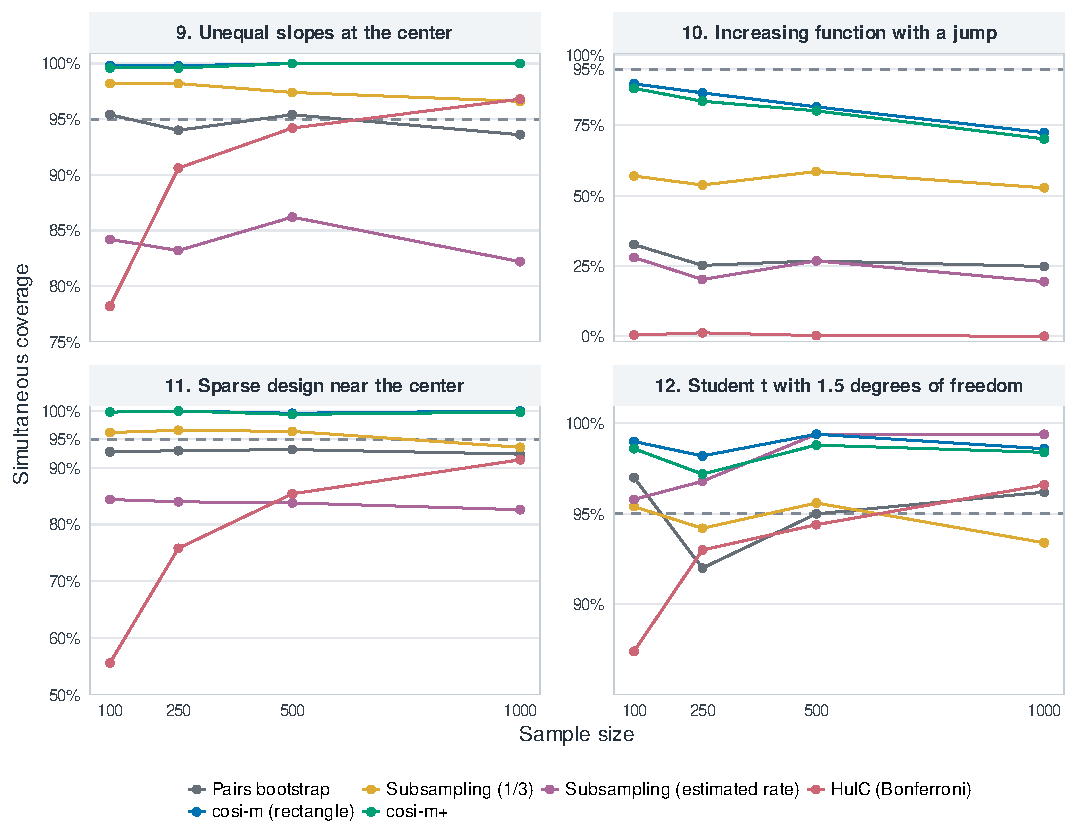
\includegraphics[width=\linewidth]{empirical_coverage_group_3.pdf}
\caption{Empirical simultaneous coverage for settings 9--12. The same data are
used for all methods within each of 500 replications at every sample size.
The dashed line marks the nominal $95\%$ level. Panel-specific vertical
limits retain all coverage values. Each rectangle is extended using the same
monotone envelope; every anchor is checked when recording coverage.}
\label{fig:coverage-3}
\end{figure}

\FloatBarrier
\section{Band-width comparisons}
\begin{figure}[h]\centering
\includegraphics[width=\linewidth]{width_ratios_group_1.pdf}
\caption{Paired ratios of average band width to the HulC width from the same
data, for settings 1--4. Both average widths are measured on $[0.1,0.9]$.
The vertical axis is logarithmic and displays $[1/16,8]$; the dashed line is one.
Boxplot statistics are computed before restricting the displayed range.
Outlier points are omitted. Companion figures display boxplots of absolute
band width.}
\end{figure}

\begin{figure}[h]\centering
\includegraphics[width=\linewidth]{width_ratios_group_2.pdf}
\caption{Paired ratios of average band width to the HulC width from the same
data, for settings 5--8. Both average widths are measured on $[0.1,0.9]$.
The vertical axis is logarithmic and displays $[1/16,8]$; the dashed line is one.
Boxplot statistics are computed before restricting the displayed range.
Outlier points are omitted. Companion figures display boxplots of absolute
band width.}
\end{figure}

\begin{figure}[h]\centering
\includegraphics[width=\linewidth]{width_ratios_group_3.pdf}
\caption{Paired ratios of average band width to the HulC width from the same
data, for settings 9--12. Both average widths are measured on $[0.1,0.9]$.
The vertical axis is logarithmic and displays $[1/16,8]$; the dashed line is one.
Boxplot statistics are computed before restricting the displayed range.
Outlier points are omitted. Companion figures display boxplots of absolute
band width.}
\end{figure}

\FloatBarrier
\section{Empirical sign diagnostics}
\begin{figure}[h]\centering
\includegraphics[width=\linewidth]{median_balance_group_2.pdf}
\caption{Fraction of the $9\times500=4500$ inference-block isotonic estimates
above $f_0(t)$ at each anchor, for settings 5--8. Each curve corresponds to a
total sample size, with half used for the pilot and half for the nine inference
blocks. The dashed line marks one half. These finite-sample diagnostics show
where the split estimates tend to lie above or below the target; they do not
impose an asymptotic symmetry conclusion.}
\end{figure}

\begin{figure}[h]\centering
\includegraphics[width=\linewidth]{median_balance_group_3.pdf}
\caption{Fraction of the $9\times500=4500$ inference-block isotonic estimates
above $f_0(t)$ at each anchor, for settings 9--12. Each curve corresponds to a
total sample size, with half used for the pilot and half for the nine inference
blocks. The dashed line marks one half. These finite-sample diagnostics show
where the split estimates tend to lie above or below the target; they do not
impose an asymptotic symmetry conclusion.}
\end{figure}

\FloatBarrier
\section*{Reproducibility materials}
The companion code and data reproduce the simulation, numerical summaries,
and figures. The full simulation is invoked from the extracted code directory by
\begin{verbatim}
source("simulation_isotonic_example.R")
study <- run_isotonic_study(core_dir=".",
  output_dir="isotonic_results")
\end{verbatim}
The script \texttt{plot\_isotonic\_saved\_results.R} regenerates the figures
from the recorded CSV files without rerunning the simulations. Computation
supports forked workers on Linux and macOS and serial execution with
\texttt{workers=1} on Windows. An optional C implementation accelerates
isotonic fitting, with a base-R implementation available as a fallback.
The results include package versions, random seeds, settings, and source
hashes. The univariate calibration functions are taken without modification
from COSI commit \texttt{3d4bcaa3f2099ae0348c481e1ba203315a78af8c}.

\bibliographystyle{plainnat}
\bibliography{isotonic_references}
\end{document}
